\section*{Money Box}

\textbf{Выполнили:}

Бочкарев Федор, Б01-003 -- электроника и программирование

Бочкарева Софья, Б01-003 -- 3D-моделирование и проектирование

\subsection {Общее описание}

Копилка со счетчиком монет. В монетной щели расположена клиновидная задвижка, присоединенная к шаговому мотору и фототранзистору. С помощью фототранзистора фиксируется наличие/отсутствие монеты в щели, а ее номинал определяется по повороту шагового мотора.

Данные о принятых монетах выводятся на дисплей в двух режимах: общая сумма в копилке и распределение содержимого по номиналам.

\subsection {Анализ существующих аналогов}

Копилки со счетчиками монет в различных вариациях представлены на маркетплейсах(https://www.ozon.ru/product/yilijukj-kopilka-dlya-deneg-11h20-sm-1358489566/?asb=sCr1GmIlWB7Fjby%252BPYnWUNFeAjvdIw5ordlD0iRvbOM%253D&asb2=sn4m9gpYWZy_EEZH7OfMzDGoCOjFWmDehfvE83sshNuqVbbHLKnkaqdBme_UnwQL9zPGT5WB-Cli3HsA9FpOcg&avtc=1&avte=2&avts=1717862839&keywords=копилка+счетчик), https://aliexpress.ru/item/1005002928697666.html?sku_id=12000028995331515&spm=a2g2w.productlist.search_results.1.5d644f98Nvin2D, 
однако такие устройства либо не являются автоматическими[1], и требуют ручного ввода добавленной суммы; либо их цена сильно завышена[2].

Определять номинал монеты можно по одному из трех признаков: диаметр, толщина или состав (магнитные свойства). Определение номинала по магнитным свойствам возможно только с очень чувствительными (дорогими) датчиками. Определение номинала по толщине требует высокой точности -- до 0,01 мм. Разница в диаметрах монет составляет минимум 1 мм. Поэтому реализовать механизм определения номинала монеты целесообразнее именно по диаметру.

Пример устройства, реализующего такой механизм, выполнен AlexGyver [](https://www.youtube.com/watch?v=lH4qfGlK2Qk). В данной идее диаметр определялся по интенсивности инфракрасного сигнала, приходящего на фоточувствительный элемент (фототранзистор).  Такая реализация допускает возможность ошибки за счет проскакивания монеты и неправильного считывания ее диаметра. К тому же в этой версии не предусмотрены удобные элементы управления (кнопки reset/переключение дисплея).

Другими аналогичными устройствами являются многочисленные реализации сортировщиков монет, основанные на проскакивании монет через щели определенного диаметра [] []. Такие устройства обладают высокой скоростью сортировки и счета, однако механизм занимает достаточно много места. Эта реализация хорошо подходит для промышленного использования (большого оборота монет), поэтому существует широкий сегмент подобных устройств, обладающих высокой надежностью и, соответственно, высокой ценой. 

Таким образом, наше устройство выделяется на фоне существующих непромышленных аналогов автоматической и надежной работой, что делает его удобным в использовании.

\subsection {Проектирование и изготовление}

Основные этапы работы:

\begin{itemize}
	\item Проектирование и прототипирование; 
	\item Изготовление деталей;
	\item Сборка;
	\item Разработка управляющей программы
\end{itemize}

\section {Проектирование и изготовление}

Основные этапы работы:

\begin{itemize}
	\item Проектирование и прототипирование; 
	\item Изготовление деталей;
	\item Сборка;
	\item Разработка управляющей программы
\end{itemize}

\subsection{Проектирование и прототипирование}

\begin{figure}[H]
	\centering
	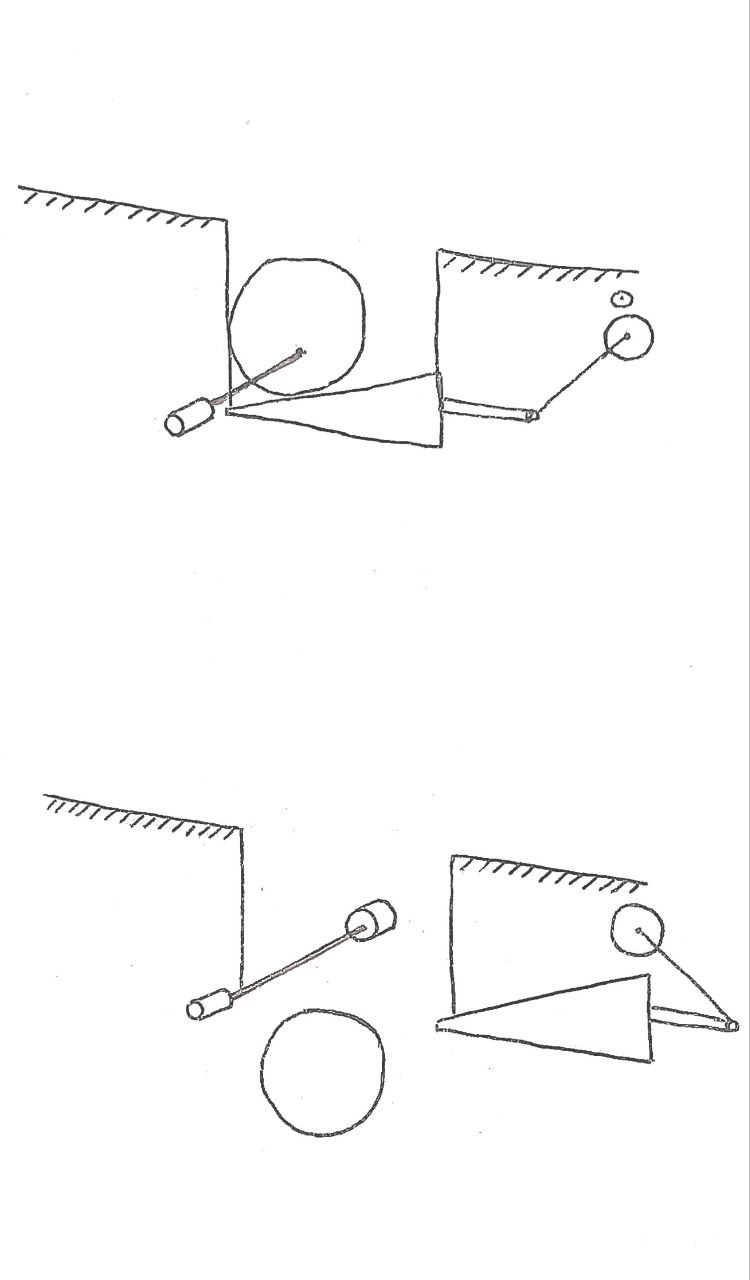
\includegraphics[width=12cm]{scheme_idea.jpg}
	\caption{Принципиальная схема устройства}
	\label{ris:scheme_idea}
\end{figure}
\par\medskip

Принципиальная схема устройства приведена на рис.~\ref{ris:scheme_idea}. Монета падает в щель монетоприемника 1 и перекрывает инфракрасный луч от инфракрасного светодиода 2. Фоторанзистор 5 передает управляющий сигнал на шаговый мотор 3, который приводит в движение клин 4. Когда клин отводится достаточно для того, чтобы монета упала насквозь, инфракрасный луч светодиода 2 перестает перекрываться, что фиксируется фототранзистором. 



По данной принципиальной схеме был собран прототип (см. рис.~\ref{ris:proto}). Он успешно прошел проверку на работоспособность, что позволило нам использовать данный механизм в дальнейшем.

\begin{figure}[H]
	\centering
	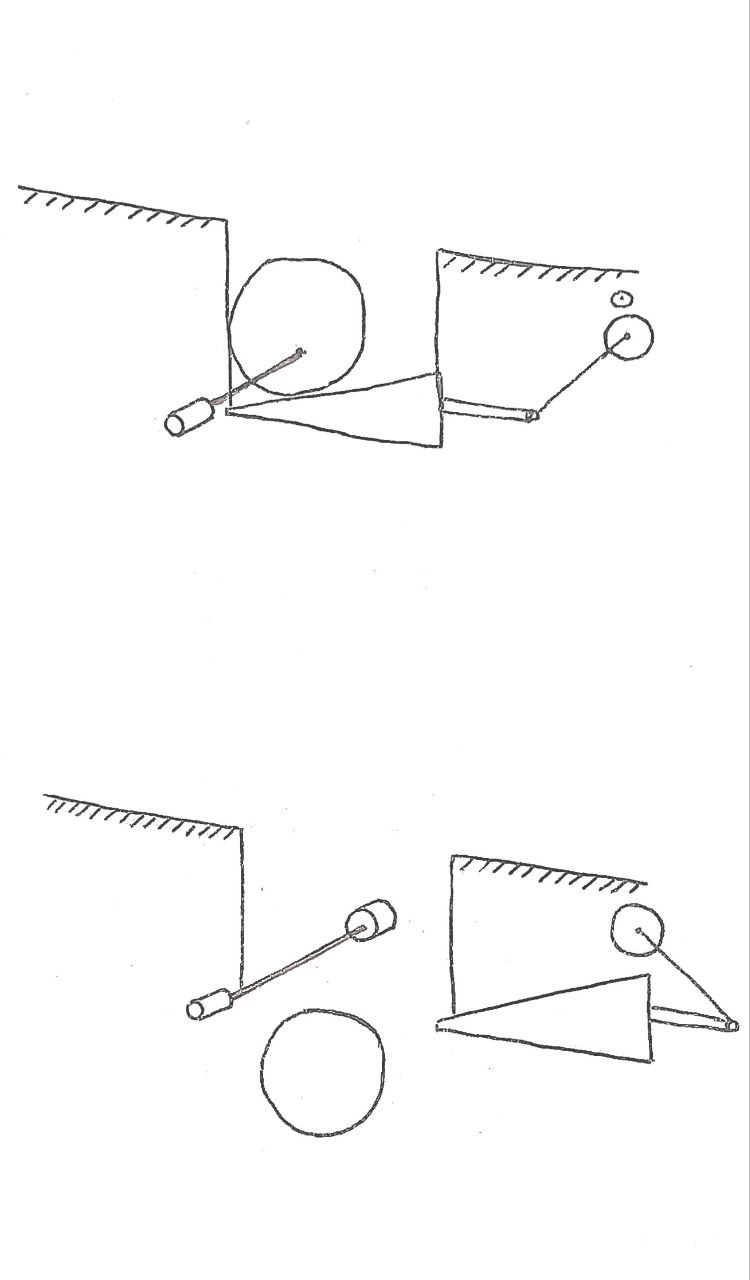
\includegraphics[width=12cm]{scheme_idea.jpg}
	\caption{Принципиальная схема устройства}
	\label{ris:scheme_idea}
\end{figure}
\par\medskip

При проектировании финальной версии мы доработали механизм затвора для его длины (со 120 мм до 60 мм) (см. рис.~\ref{ris:mechan}).
Корпус копилки состоит из двух основных составных частей - крышки, на которой закреплены все основные детали механизма, и коробки для монет (см. рис.~\ref{ris:korob}). 

\begin{figure}[H]
	\centering
	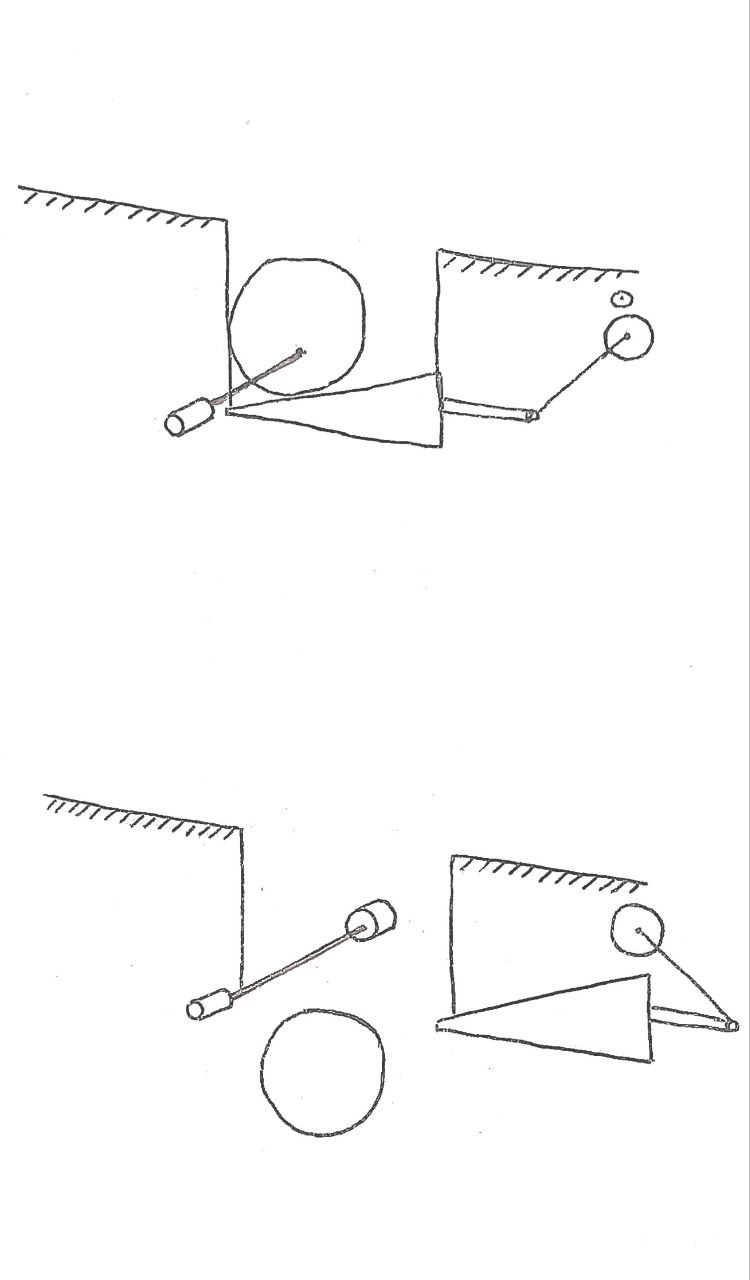
\includegraphics[width=12cm]{scheme_idea.jpg}
	\caption{Принципиальная схема устройства}
	\label{ris:scheme_idea}
\end{figure}
\par\medskip

На верхней крышке предусмотрено размещение 2-х кнопок, дисплея, модуля Arduino Nano, драйвера шагового мотора и его драйвера, фототранзистора и инфракрасного светодиода и механизма затвора. Питание осуществляется от постоянного тока 5V от сети (см. рис.~\ref{ris:kryshka}).  

\begin{figure}[H]
	\centering
	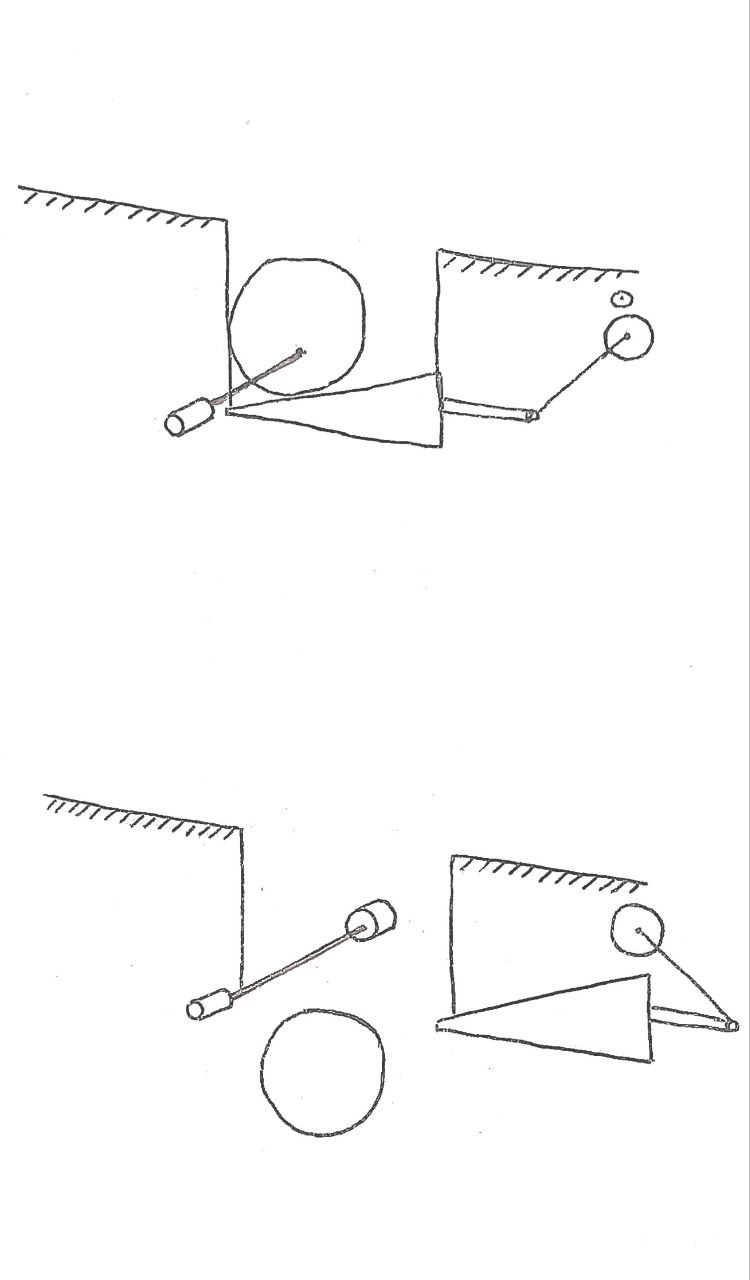
\includegraphics[width=12cm]{scheme_idea.jpg}
	\caption{Принципиальная схема устройства}
	\label{ris:scheme_idea}
\end{figure}
\par\medskip
\subsection{Изготовление и сборка.}

Все детали были изготовлены на 3д принтере. Изначально коробка была сделана без ребер жесткости, из-за чего при печати она деформировалась. Поэтому мы изменили конструкцию коробки, добавив ребра жесткости. 
\par\medskip

\begin{figure}[H]
	\centering
	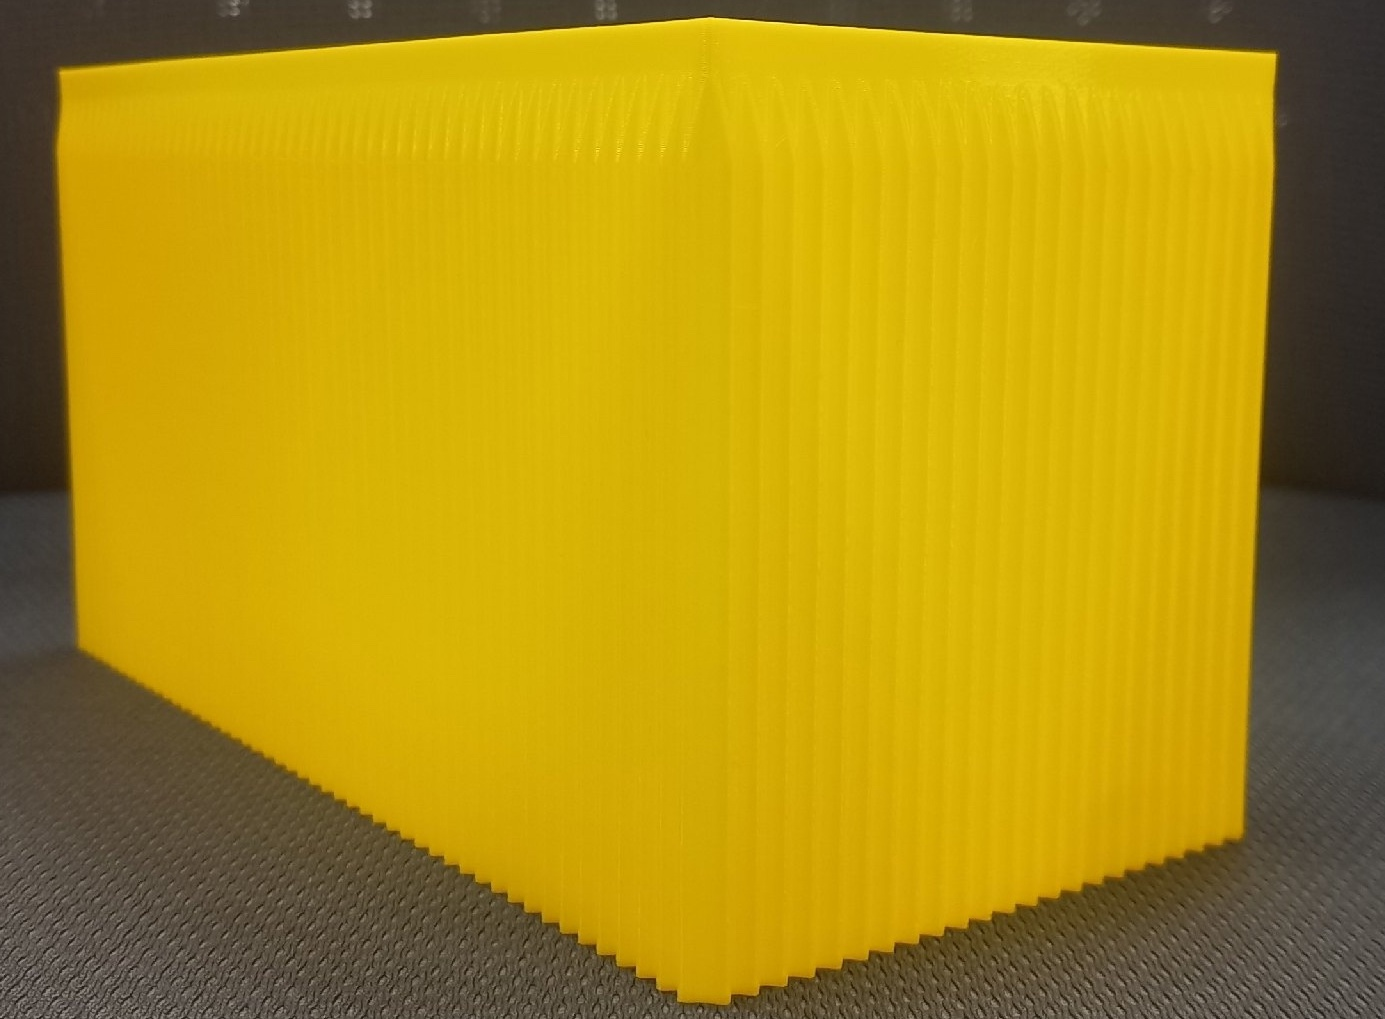
\includegraphics[width=12cm]{pics/korob.jpg}
	\caption{Короб для монет}
	\label{ris:korob_done}
\end{figure}

Электрическая схема была собрана из: шагового мотора, платы-драйвера шагового мотора, Arduino Nano, фототранзистора, ИК-светодиода, LCD экрана формата 2004 вместе с платой I2C, 2-х кнопок и провода USB (для питания). Схема соединений приведена ниже на рисунке~\ref{ris:scheme_electric}.

\begin{figure}[H]
	\centering
	\includegraphics[width=12cm]{pics/scheme_png.png}
	\caption{Схема соединения проводов}
	\label{ris:scheme_electric}
\end{figure}

При сборке были исправлены выявленные ошибки моделирования. В основном это касается отсутствующего отверстия для щели под ИК-светодиод и фототранзистор.
\par\medskip
\subsection{Сборка}

Основным этапом стала сборка итогового устройства.
\par\medskip

Электрическая схема была собрана из: шагового мотора, платы-драйвера шагового мотора, Arduino Nano, фототранзистора, ИК-светодиода, LCD экрана формата 2004 вместе с платой I2C, 2-х кнопок и провода USB (для питания). Схема соединений приведена ниже на рисунке~\ref{ris:scheme_electric}.

\begin{figure}[H]
	\centering
	\includegraphics[width=12cm]{scheme_png.png}
	\caption{Схема соединения проводов}
	\label{ris:scheme_electric}
\end{figure}

При сборке были исправлены выявленные ошибки моделирования. В основном это касается отсутствующего отверстия для щели под ИК-светодиод и фототранзистор.
\par\medskip

В ходе процесса калибровки открытия щели для определенного номинала монет, была многократно доработана система задвижки -- методом перебора были отсеяны 2 наиболее подходящие пружины из порядка 20 оставшихся и одна из них была растянута/раскручена для достижения надёжной работы механизма.
\par\medskip

С ходе испытаний, шаговый мотор смог провернуть стопорное положение (упор в корпус) и тем самым деформировал стенку корпуса. Для восстановления работоспособности механизма задвижки корпус крышки был незначительно дефформирован -- была вставлена насквозь в стенку в месте упора небольшой штырёк, обеспечивающий надёжное стопорное положение для шагового мотора.

\subsubsection{Разработка управляющей программы}

Привести код, объяснить код. 

\subsection {Тестирование}

\subsection {Результаты}

\subsection {Структуры Scoreboarding}

\begin{figure}[H]
	\centering
	\includegraphics[width=12cm]{try.jpg}
	\caption{Рис.1. Пример программного использования команд блокировки LL и SC}
	\label{fig:p_chest}
\end{figure}
\par\medskip

Также существуют \textbf{Спин-блокировки}, использующие когерентность. Блокировки в кэше обладают преимуществами более быстрого процесса и локальности блокировок (возможность повтора операции синхронизации) (см. рис. 2).

\begin{figure}[H]
	\centering
	\includegraphics[width=12cm]{spin.jpg}
	\caption{Рис.2. Пример спин-блокировки}
	\label{fig:p_chest}
\end{figure}
\par\medskip